%\onecolumn

\section{Experiments}
	\subsection{Finding the Wavelength}

\emph{NOTE: Do not send square waves or frequencies greater than 100Hz
to the Piezo, as this may result in damage.}

\begin{enumerate}
 	\item Set the function generator to a low frequency sinusoid.
		\begin{figure}[ht!]
		\centering
		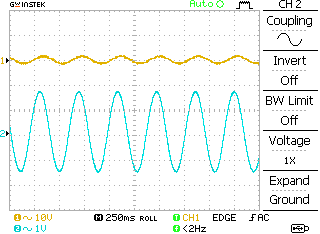
\includegraphics[width=2in]{DS0000}
		\end{figure}
	\item Connect the function generator's output to the oscilloscope's CH2
        and the Piezo via a T-connector.
	\item Using the scope, calculate the voltage difference required
		  to move the mirror through one complete fringe.
		\begin{figure}[ht!]
		\centering
		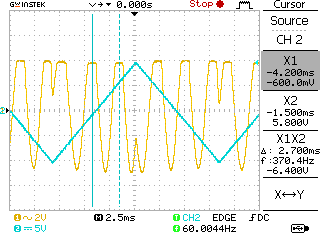
\includegraphics[width=2in]{DS0007}
		\end{figure}

	\emph{NOTE: Due to the mismatch in impedance (most function generators
		are 50 Ohm impedence), the amplitude seen by the piezo and scope is closer to 20 Vpp.}
	
	\item Press the \emph{Cursor} button to get the cursors on the oscilloscope screen and set it so the input is CH 2.
	\item Record the maximum intensity of the interferometer by moving the first cursor to the highest point of the fringes.
	\item Record the lowest intensity of the interferometer by moving the second cursor to the lowest point of the fringes.
	\item Get an image of the oscilloscope screen by pressing the \emph{Run/Stop} button. 
	\item Record the difference in voltage from one trough to the next. 
	
	\emph{Be careful not to take a measurement from the trough near or on a peak of the ramp function.}
	
	\item Repeat previous step 7 more times for one set of 8 measurements. 
	\item Calculate the average of the voltage differences.
	\item Do this for a second set.
	\item Calculate the average of the voltage differences for each set.
\end{enumerate}



\textbf{Question 1:}
	\indent What is the visibility of the interferometer?
	
\textbf{Question 2:}
	\indent If the piezo moves 6.1 $\mu$m per 100 Volts and $D=\frac{\lambda}{2}$, what is the wavelength of the laser?
	
\textbf{Question 3:}
	\indent Why would the fringe pattern change when you hit or lean on the table?
% measure voltages thru one complete fringe change. add picture. take multiple measurements, using run/stop command.

